As mentioned in the \ref{sec:Problem_Analysis} the best spot of the execution to parallelize is the frontier scanning, this due to its huge size in most of graphs. To achieve this has been used a \textbf{farm pattern} in which the frontier is splitted among all the workers by an \textbf{emitter} and the results of worker computation are merged in a new frontier by a \textbf{collector}.
In all the following solutions the $nw$ is intended only as the number of workers in the farm, so are not considered the emitter and collector threads.
\subsection{C++ STL Solutions}
\label{subsec:CStatic}
\subsubsection{Static Scheduling}
In this section will be described in details the solution with the static scheduling of the frontier's chunks.
The execution starts with the initialization of the farm: an emitter, a vector of workers and a collector are created. In addition to this, are initialized all data structures for level analysis and synchronization. In particular, for communication, each worker has a queue where the emitter distributes chunk ranges. On the other hand, the data are retrieved from the farm exploiting shared references of the workers' new frontier with the collector.

With this approach, the emitter divides the frontier $F$ size by the number of workers ($nw$), then creates the pairs in which are present start and the end position of the chunk. These pairs are pushed in the worker's queue that extracts it and starts to work on his chunk. To avoid that the emitter execution restart a condition variable has been used to put the emitter thread in a wait state. 
Popped the chunk from the queue, the worker starts to iterate on the frontier in its range. For each node, firstly checks if the vertex has already been visited exploiting the $compare\_and\_exchange$ that allows to perform both fetch and update operations in an atomic fashion. The method returns true if it was able to change the state of the node to visit, otherwise, it is skipped.
In the case of a positive outcome, the analysis of the node continues by checking the value associated with it and visiting its list of neighbors. During this list iterations, is verified if the neighbor has been already added in the next frontier vector by another worker.
To synchronize the farm with the collector the workers perform a $fetch\_add$ operation on an atomic variable $end\_of\_task$, when it reaches $nw$ the collector operations start. In this phase all the workers' next frontiers are merged in $F'$, the old frontier $F$ gets cleared and swapped with $F'$. In addition, the condition variable state is changed to allow emitter restart. These three steps are repeated until the collector's next frontier is empty, in this case in the frontier is pushed a special node $Stopper$ received by the emitter that blocks the worker using $Stop\_exe$ pairs. When the worker receives this pair atomically fetch and add the local counter of the found occurrences to a shared counter.

\begin{figure}[htb!]
    \centering
    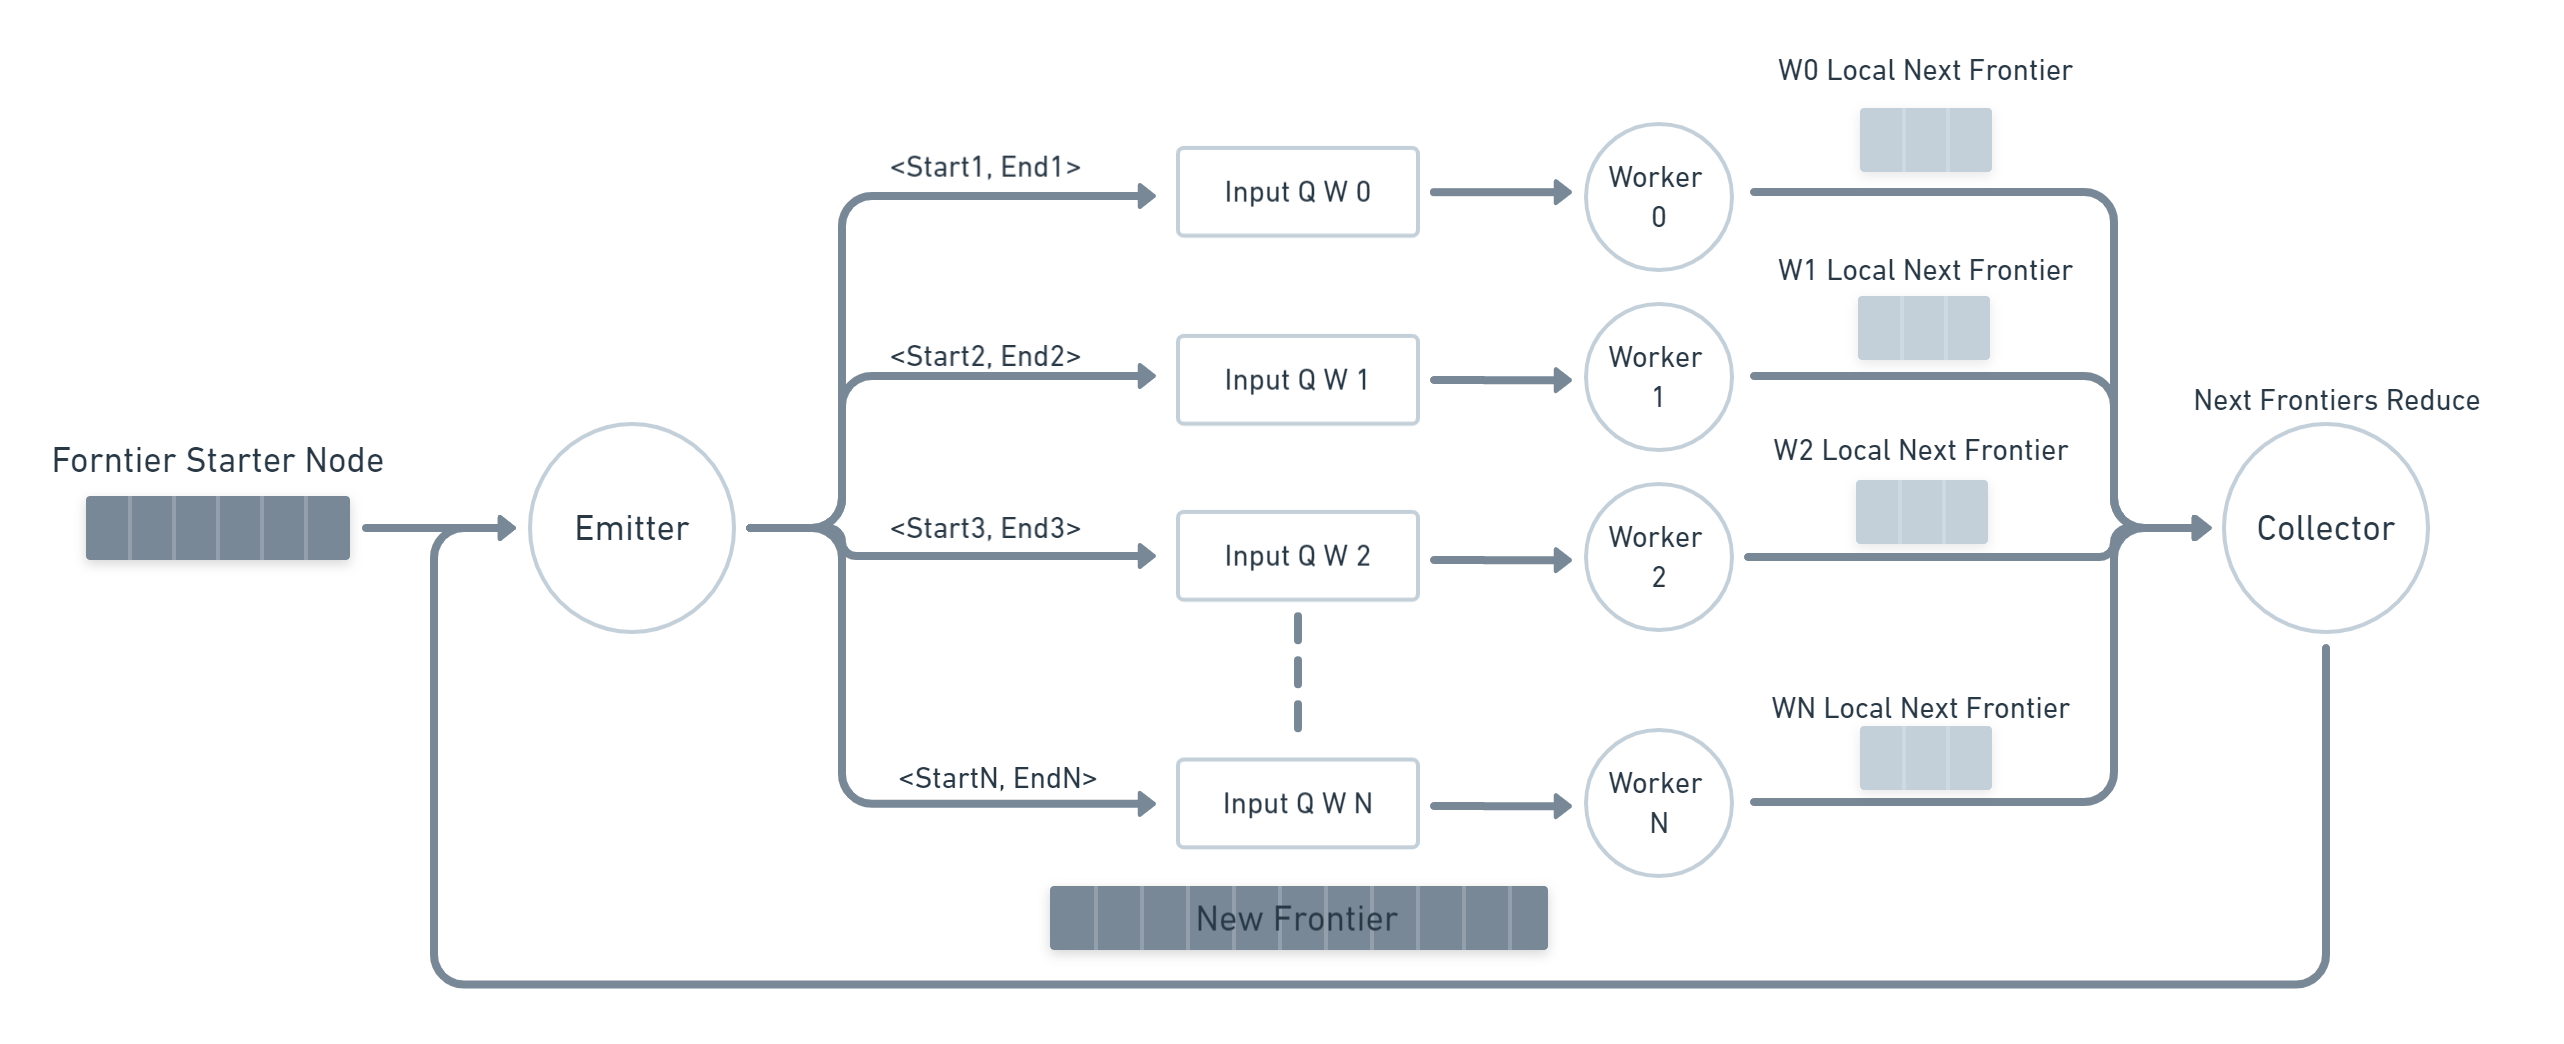
\includegraphics[width=0.95\textwidth]{Figures/par_schema.png}
    \caption{Schema of the static scheduling solution.}
    \label{fig:bfs_par_1_schema}
\end{figure}
\FloatBarrier

The main problem of this approach is the load balancing mostly in the cases in which the graph is highly connected. In this scenario, the worker that gets the first chunk has the possibility to visit a large section of the graph and so makes the visit of the other workers faster and creates a bottleneck due to the necessity of waiting for the first worker to finish the visit its portion making the service time of the farm becomes $T_{farm} = max\{T_{w_1}, T_{w_2}, ..., T_{w_n}\}$.  
This can be seen in the tables \ref{table:sched_st1} and \ref{table:sched_st2}.


\begin{table}[htb!]
\centering
\begin{tabular}{l|c|c|c|}
\cline{2-4}
\multicolumn{1}{c|}{}                  & Worker 1 & Worker 2 & Worker 3 \\ \hline
\multicolumn{1}{|l|}{Time ($\mu sec$)}             & 103925    & 62256    & 14293     \\ \hline
\multicolumn{1}{|l|}{Discovered nodes} & 2048     & 1429     & 1514     \\ \hline
\end{tabular}
\caption{Load balancing of analysis, with static scheduling, of the first frontier, size 5013, graph 10K 0.5 density}
\label{table:sched_st1}
\end{table}


\begin{table}[htb!]
\centering
\begin{tabular}{l|c|c|c|}
\cline{2-4}
\multicolumn{1}{c|}{}                  & Worker 1 & Worker 2 & Worker 3 \\ \hline
\multicolumn{1}{|l|}{Time ($\mu sec$)}             & 6685    & 5137    & 2971     \\ \hline
\multicolumn{1}{|l|}{Discovered nodes} & 1579     & 461     & 109     \\ \hline
\end{tabular}
\caption{Load balancing of analysis, with static scheduling, of the second frontier, size 7121 nodes, graph 10K 0.02 density}
\label{table:sched_st2}
\end{table}
\FloatBarrier

\subsubsection{Dynamic Scheduling}
To better manage the load balancing between threads and to avoid the possibility that the first worker explores most of the graph a solution can be to divide the frontier into smaller chunks to reduce the visibility of the graph to workers. Due to these changes, the scheduling policy has been changed in favor of a dynamic load balancing handled by a shared task queue $Q$. Another consequence is the addition of an additional input parameter, $chunk_size$. This value is used by the emitter to create the new range pairs. By increasing the number of chunks to be generated, increases the work of the emitter and consequently its time $T_e$, introducing more overhead. To preserve the solution performance, the workers extract the new chunks as soon as they are available in the shared queue.
To monitor the execution, also in this case, is used the $end\_of\_task$ variable that keeps track of all generated chunks: the emitter increments it for each new pair pushed in the $Q$ and the workers decrements it for each popped one when it reaches $0$ the collector is triggered.


\begin{figure}[htb!]
    \centering
    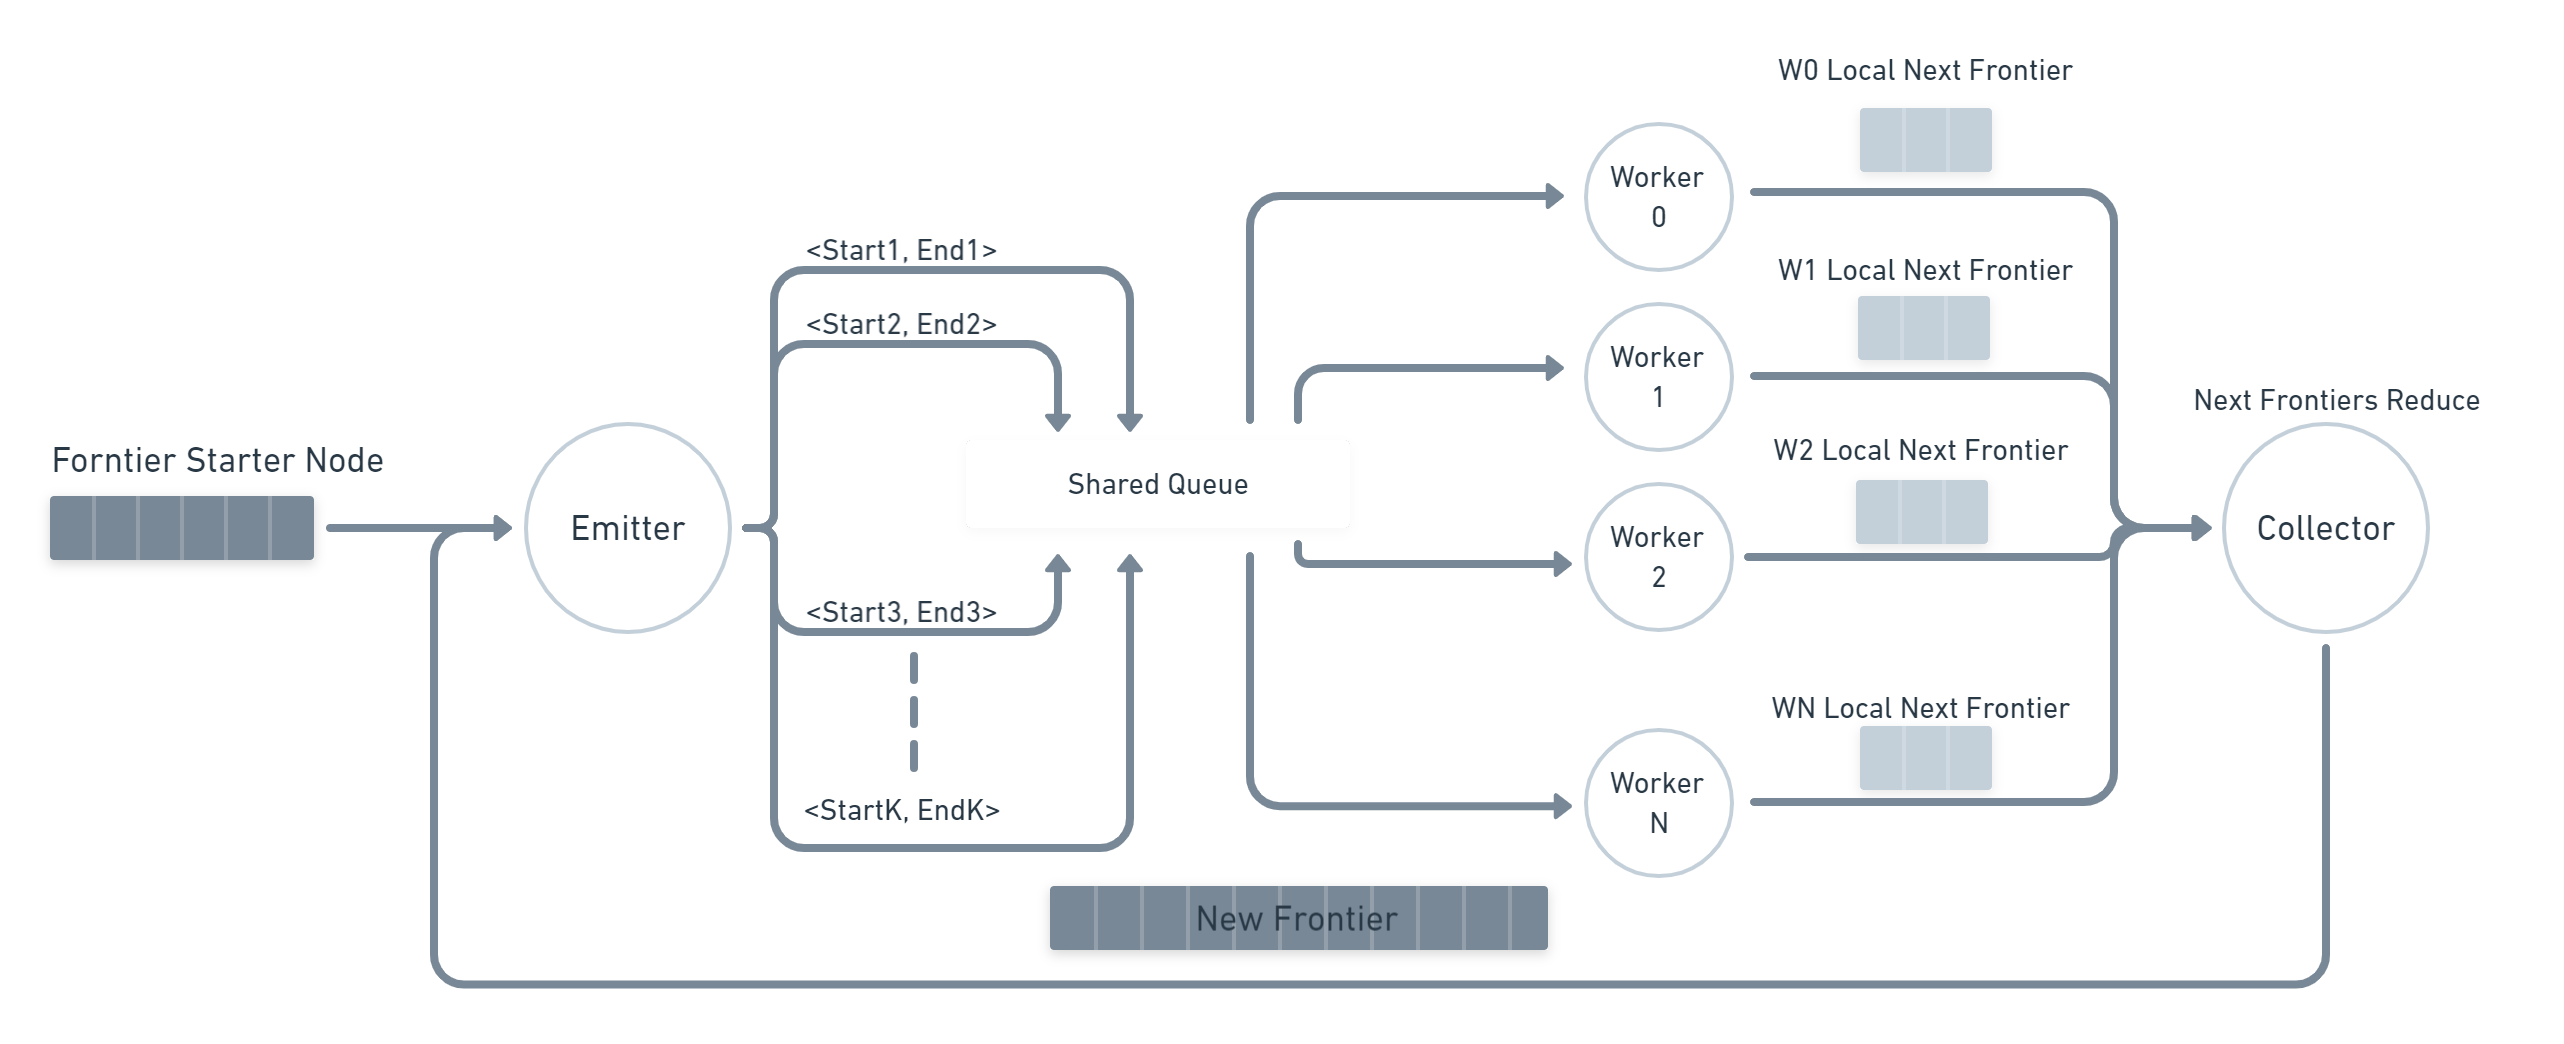
\includegraphics[width=0.95\textwidth]{Figures/par_dy.png}
    \caption{Schema of the dynamic scheduling solution.}
    \label{fig:bfs_par_2_schema}
\end{figure}
\FloatBarrier

Using a dynamic approach for task management the load balancing is distributed evenly across threads as can be seen in the table \ref{table:sched_dy}.
\label{table:sched_dy}
\begin{table}[htb!]
\centering
\begin{tabular}{l|c|c|c|}
\cline{2-4}
\multicolumn{1}{c|}{}                  & Worker 1 & Worker 2 & Worker 3 \\ \hline
\multicolumn{1}{|l|}{Time ($\mu sec$)}             & 23121    & 23376    & 22797    \\ \hline
\multicolumn{1}{|l|}{Discovered nodes} & 2543     & 3376     & 578      \\ \hline
\end{tabular}
\caption{Load balancing of analysis, with dynamic scheduling, of the first frontier graph 10K 0.5 density}
\end{table}

The considerable gain in terms of load balancing removing the bottlenecks in the execution of the farm is counterbalanced by a increase time of the emitter $T_e$, as can been seen in the following tables \ref{table:emit_coll} and \ref{table:emit_coll_dy}. The chunk size plays an important role, indeed, having small chunks improves the load balancing but the splitting time would increase dramatically, so it's important to find the trade-off. In addition, For large chunk sizes, in the case of small tiers, it might be possible to generate less than $nw$ portions and thus not fully exploit the farm.

\begin{table}[!htb]
\centering
\begin{minipage}{0.08\textwidth}
\centering
\begin{tabular}{|c|}
\hline
NW \\ \hline
1          \\ \hline
2      \\ \hline
4           \\ \hline
8            \\ \hline
16       \\ \hline
32          \\ \hline
\end{tabular}
\end{minipage}
\begin{minipage}{0.43\textwidth}
\centering
\begin{tabular}{|c|c|c|}
\hline
 10K 0.02D & 10K 0.5D & 10K 0.8D \\ \hline
 398       & 411      & 552      \\ \hline
905       & 325      & 47       \\ \hline
 1299      & 665      & 466      \\ \hline
1091      & 1284     & 1738     \\ \hline
1524      & 712      & 1524     \\ \hline
1631      & 1460     & 1464     \\ \hline
\end{tabular}

\end{minipage}
\begin{minipage}{0.43\textwidth}
\centering
\begin{tabular}{|c|c|c|}
\hline
 10K 0.02D & 10K 0.5D & 10K 0.8D \\ \hline
149       & 126      & 38       \\ \hline
238       & 149      & 898      \\ \hline
270       & 330      & 77       \\ \hline
290       & 171      & 77       \\ \hline
359       & 230      & 359      \\ \hline
461       & 335      & 52       \\ \hline
\end{tabular}
\end{minipage}
\caption{Total time ($\mu sec$) spend by Emitter and Collector in $\mu sec$, static solution.}
\label{table:emit_coll}
\end{table}

\begin{table}[!htb]
\centering
\begin{minipage}{0.08\textwidth}
\centering
\begin{tabular}{|c|}
\hline
NW \\ \hline
1          \\ \hline
2      \\ \hline
4           \\ \hline
8            \\ \hline
16       \\ \hline
32          \\ \hline
\end{tabular}
\end{minipage}
\begin{minipage}{0.43\textwidth}
\centering
\begin{tabular}{|c|c|c|}
\hline
10K 0.02D & 10K 0.5D & 10K 0.8D \\ \hline
1137       & 565      & 602      \\ \hline
1524       & 1091     & 899      \\ \hline
1465       & 2014     & 1131     \\ \hline
2398      & 1940      & 2120     \\ \hline
2614      & 2211     & 1047     \\ \hline
7947      & 6751     & 3645     \\ \hline
\end{tabular}
\end{minipage}
\begin{minipage}{0.43\textwidth}
\centering
\begin{tabular}{|c|c|c|}
\hline
10K 0.02D & 10K 0.5D & 10K 0.8D \\ \hline
111       & 78       & 24       \\ \hline
244       & 103      & 26       \\ \hline
211       & 102      & 49       \\ \hline
214       & 278      & 85       \\ \hline
162       & 119      & 47       \\ \hline
188       & 165      & 75       \\ \hline
\end{tabular}
\end{minipage}
\caption{Total time ($\mu sec$) spend by Emitter and Collector in $\mu sec$, dynamic solution with 32 of chunk size.}
\label{table:emit_coll_dy}
\end{table}
\FloatBarrier


\subsection{Fast Flow Solution}
The Fast Flow solution is based on the same reasoning of the first C++ STL solution (\ref{subsec:CStatic}), in particular, it has been implemented using a farm in which has been removed the collector and added for each worker feedback channel to the emitter. For data communication has been used a personalized task struct in which is present a pair that indicates the start and the end position of the chunk and a next frontier vector. Similar to the first C++ version,  the load balancing is static but in this case, the scheduling exploits the Round Robin algorithm embedded in Fast Flow.

\begin{figure}[htb!]
    \centering
    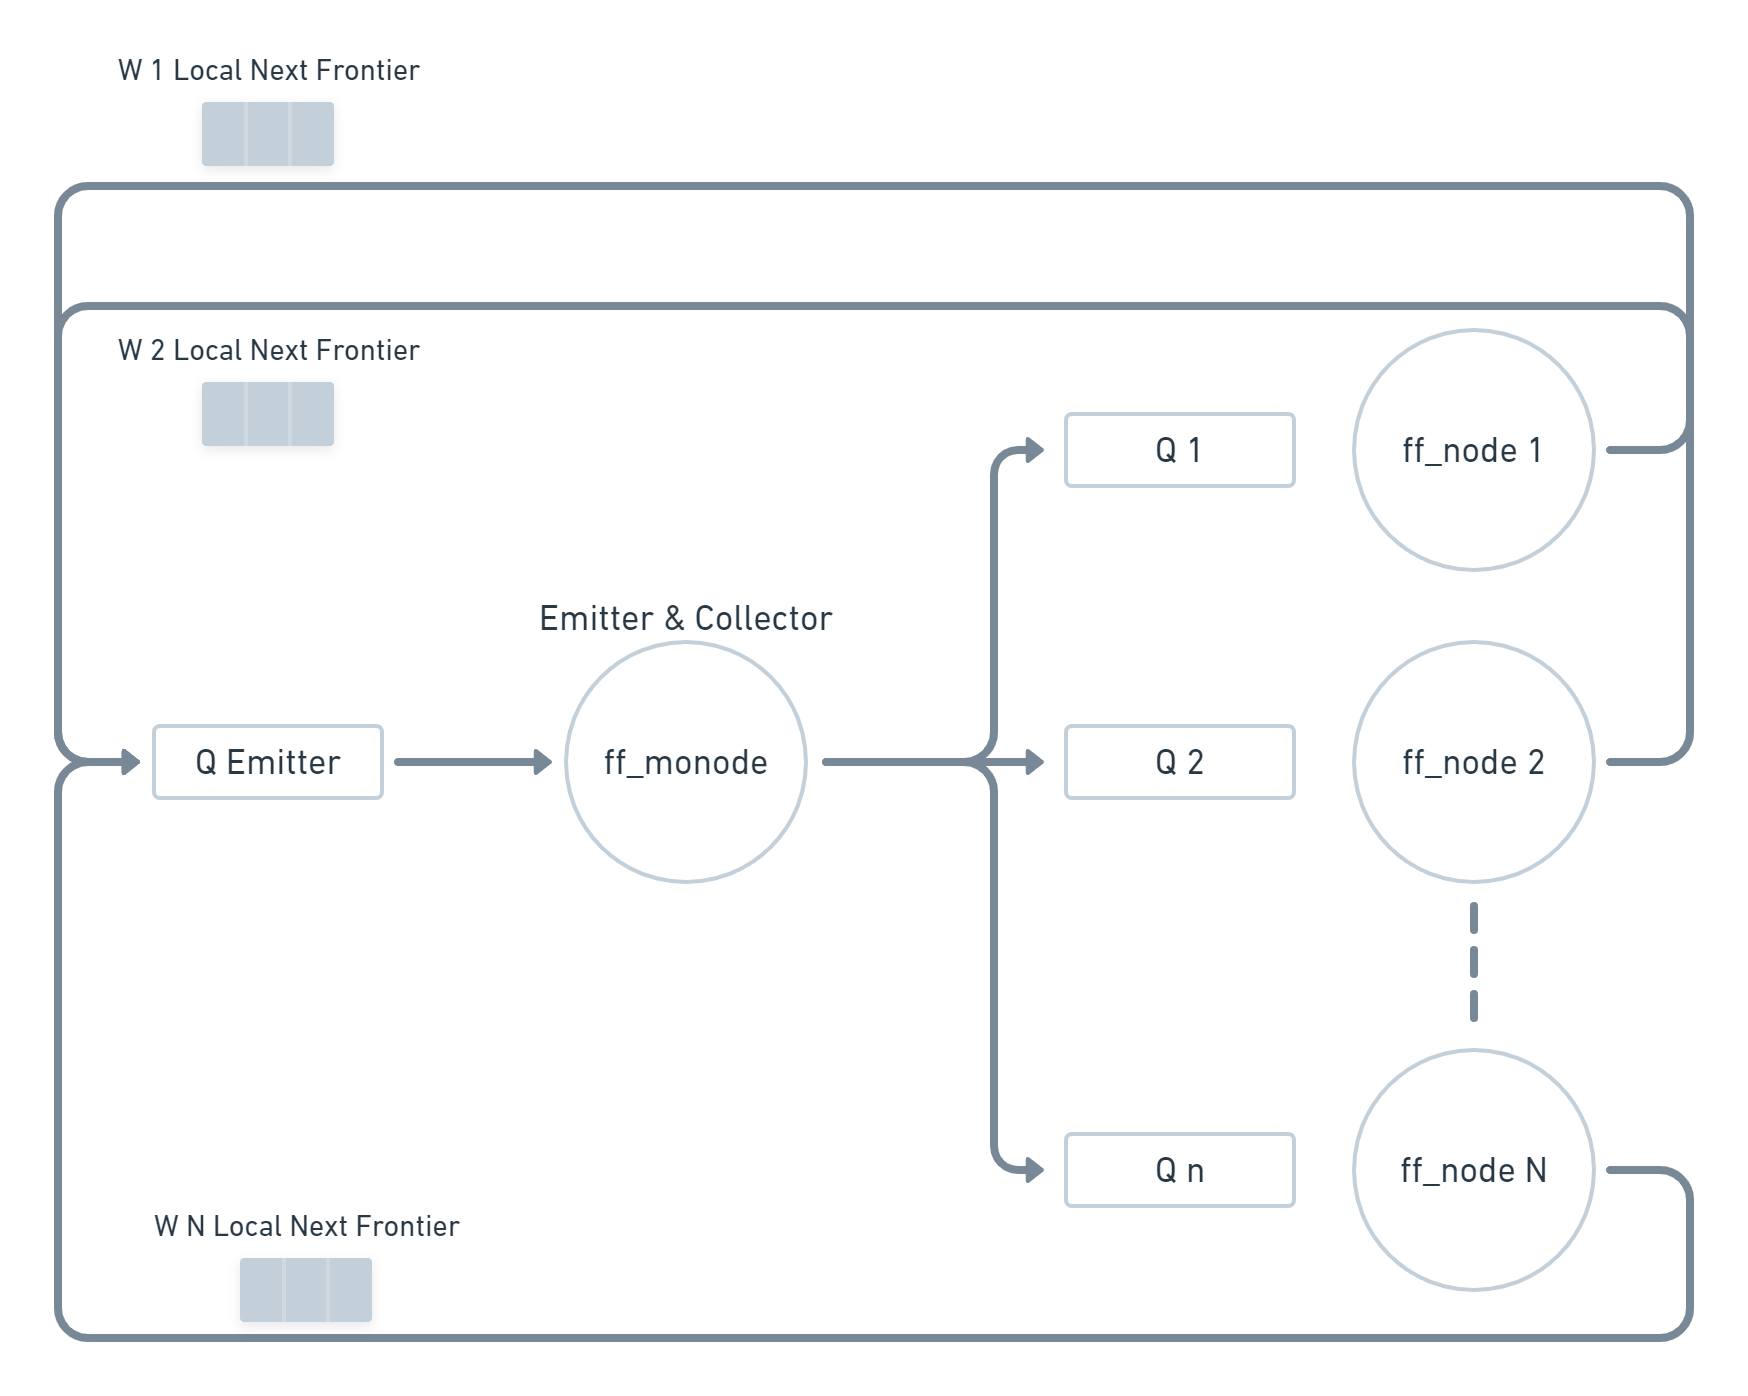
\includegraphics[width=0.55\textwidth]{Figures/FF.png}
    \caption{Schema of the Fast Flow solution.}
    \label{fig:FF}
\end{figure}
\FloatBarrier
